\documentclass[tikz,border=3mm]{standalone}
\usetikzlibrary{arrows.meta,positioning,calc}
\begin{document}
\pagecolor{white}
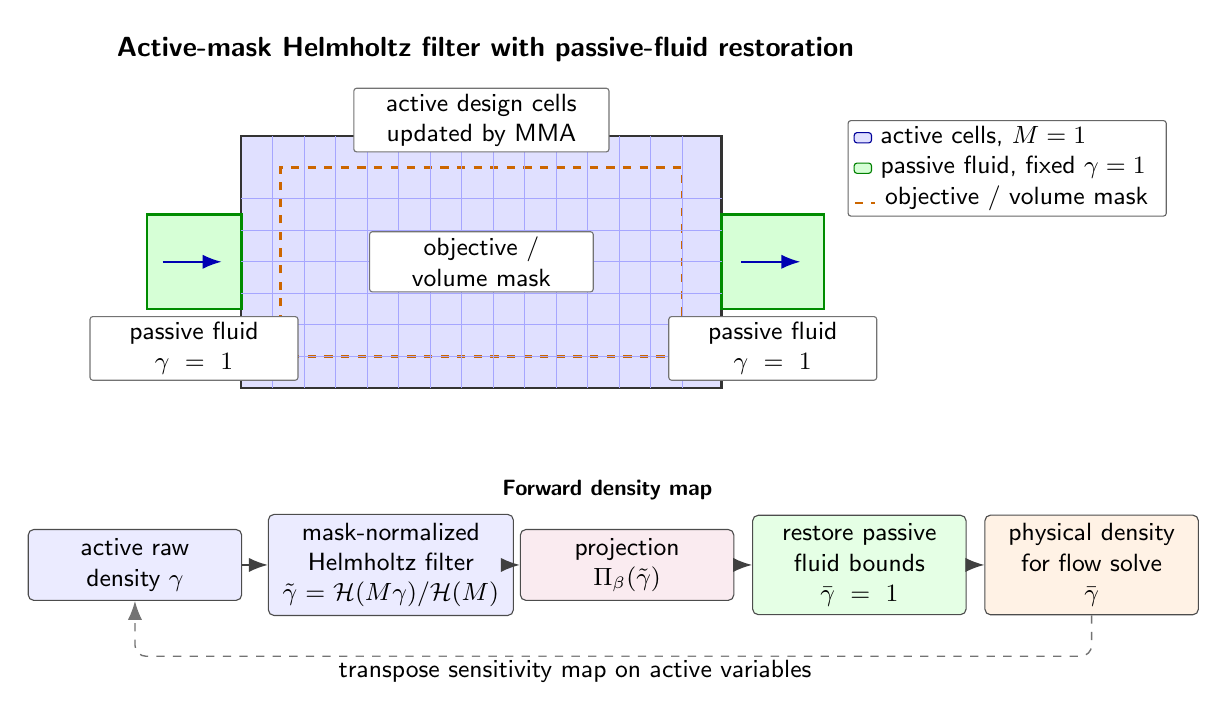
\begin{tikzpicture}[
  font=\sffamily\small,
  arrow/.style={-{Latex[length=2.4mm]}, line width=0.55pt, draw=black!75},
  backarrow/.style={-{Latex[length=2.4mm]}, line width=0.5pt, draw=black!55, dashed, rounded corners=4pt},
  box/.style={draw=black!70, rounded corners=2pt, align=center, minimum height=9mm, text width=25mm, inner sep=3pt},
  labelbox/.style={draw=black!55, fill=white, rounded corners=1pt, inner sep=2pt, align=center},
  legend/.style={draw=black!60, rounded corners=1pt, fill=white, inner sep=2pt, align=left, text width=39mm},
  active/.style={fill=blue!12, draw=blue!60!black},
  fluid/.style={fill=green!16, draw=green!50!black},
  objective/.style={draw=orange!80!black, line width=0.9pt, dashed}
]

\node[font=\sffamily\bfseries] at (4.45,4.85) {Active-mask Helmholtz filter with passive-fluid restoration};

% Domain schematic: only passive-fluid non-design regions are shown.
\fill[active] (1.35,0.55) rectangle (7.45,3.75);
\fill[fluid] (0.15,1.55) rectangle (1.35,2.75);
\fill[fluid] (7.45,1.55) rectangle (8.75,2.75);
\draw[black!80, line width=0.8pt] (1.35,0.55) rectangle (7.45,3.75);
\draw[green!55!black, line width=0.9pt] (0.15,1.55) rectangle (1.35,2.75);
\draw[green!55!black, line width=0.9pt] (7.45,1.55) rectangle (8.75,2.75);
\draw[objective] (1.85,0.95) rectangle (6.95,3.35);

% Mesh/grid hints in active cells.
\foreach \x in {1.75,2.15,...,7.05} {
  \draw[blue!35, line width=0.25pt] (\x,0.55) -- (\x,3.75);
}
\foreach \y in {0.95,1.35,...,3.35} {
  \draw[blue!35, line width=0.25pt] (1.35,\y) -- (7.45,\y);
}

\draw[arrow, blue!70!black] (0.35,2.15) -- (1.10,2.15);
\draw[arrow, blue!70!black] (7.70,2.15) -- (8.45,2.15);

\node[labelbox, text width=31mm] at (4.40,3.95) {active design cells\\updated by MMA};
\node[labelbox, text width=25mm] at (0.75,1.05) {passive fluid\\$\gamma=1$};
\node[labelbox, text width=25mm] at (8.10,1.05) {passive fluid\\$\gamma=1$};
\node[labelbox, text width=27mm] at (4.40,2.15) {objective /\\volume mask};

\node[legend, anchor=north west] at (9.05,3.95) {
  \tikz{\fill[active] (0,0) rectangle (0.22,0.13);} active cells, $M=1$\\
  \tikz{\fill[fluid] (0,0) rectangle (0.22,0.13);} passive fluid, fixed $\gamma=1$\\
  \tikz{\draw[objective] (0,0.06) -- (0.26,0.06);} objective / volume mask
};

% Filter chain.
\node[font=\sffamily\bfseries\footnotesize] at (6.0,-0.75) {Forward density map};
\node[box, fill=blue!8] (raw) at (0.0,-1.70) {active raw\\density $\gamma$};
\node[box, fill=blue!8, text width=29mm] (filter) at (3.25,-1.70) {mask-normalized\\Helmholtz filter\\$\tilde{\gamma}=\mathcal{H}(M\gamma)/\mathcal{H}(M)$};
\node[box, fill=purple!8] (proj) at (6.25,-1.70) {projection\\$\Pi_\beta(\tilde{\gamma})$};
\node[box, fill=green!10] (restore) at (9.20,-1.70) {restore passive\\fluid bounds\\$\bar{\gamma}=1$};
\node[box, fill=orange!10] (phys) at (12.15,-1.70) {physical density\\for flow solve\\$\bar{\gamma}$};

\draw[arrow] (raw) -- (filter);
\draw[arrow] (filter) -- (proj);
\draw[arrow] (proj) -- (restore);
\draw[arrow] (restore) -- (phys);

\draw[backarrow] (phys.south) -- ++(0,-0.52) -|
  node[pos=0.27, below, fill=white, inner sep=1pt] {transpose sensitivity map on active variables}
  (raw.south);

\end{tikzpicture}
\end{document}
